% ToDo: Kurze Erläuterung, weil auf dem Screenshot nicht viel erkennbar
%% Erinnerungsstütze: 
%% Gesucht hatte ich nur nach dem \hypersetup Befehl, mit welchem man die Farbe von klickbaren BibTeX-Zitationen ändert. 
%% Gemini antwortet mit dem richtigen Kommando. Hey super danke, brauche nicht lange suchen!
%% Jedoch: Hier wurden zu Ende Teile der TeX-Syntax übersetzt!
%% Zwar: Nur die Farbe, welche ich sowieso selber einstellen wollte/muss, jedoch war die gegebene beispielhafte Verwendung falsch, da sie nicht kompilierbar wäre (bzw. an sich schon, jedoch würde statt einer Farbe bei einem nicht zulässlichen String der Default-Wert verwendet werden, rgba(0,0,0,.0)). Danke an VSCode für's highlighten.
\subsection{Google Suche vom 03.10.2025}
\begin{figure}[h!tb]
    \centering
    \caption{Von der reinen Aufgabenstellung prinzipiell unabhängige Google-Suche vom 03.10.2025}
    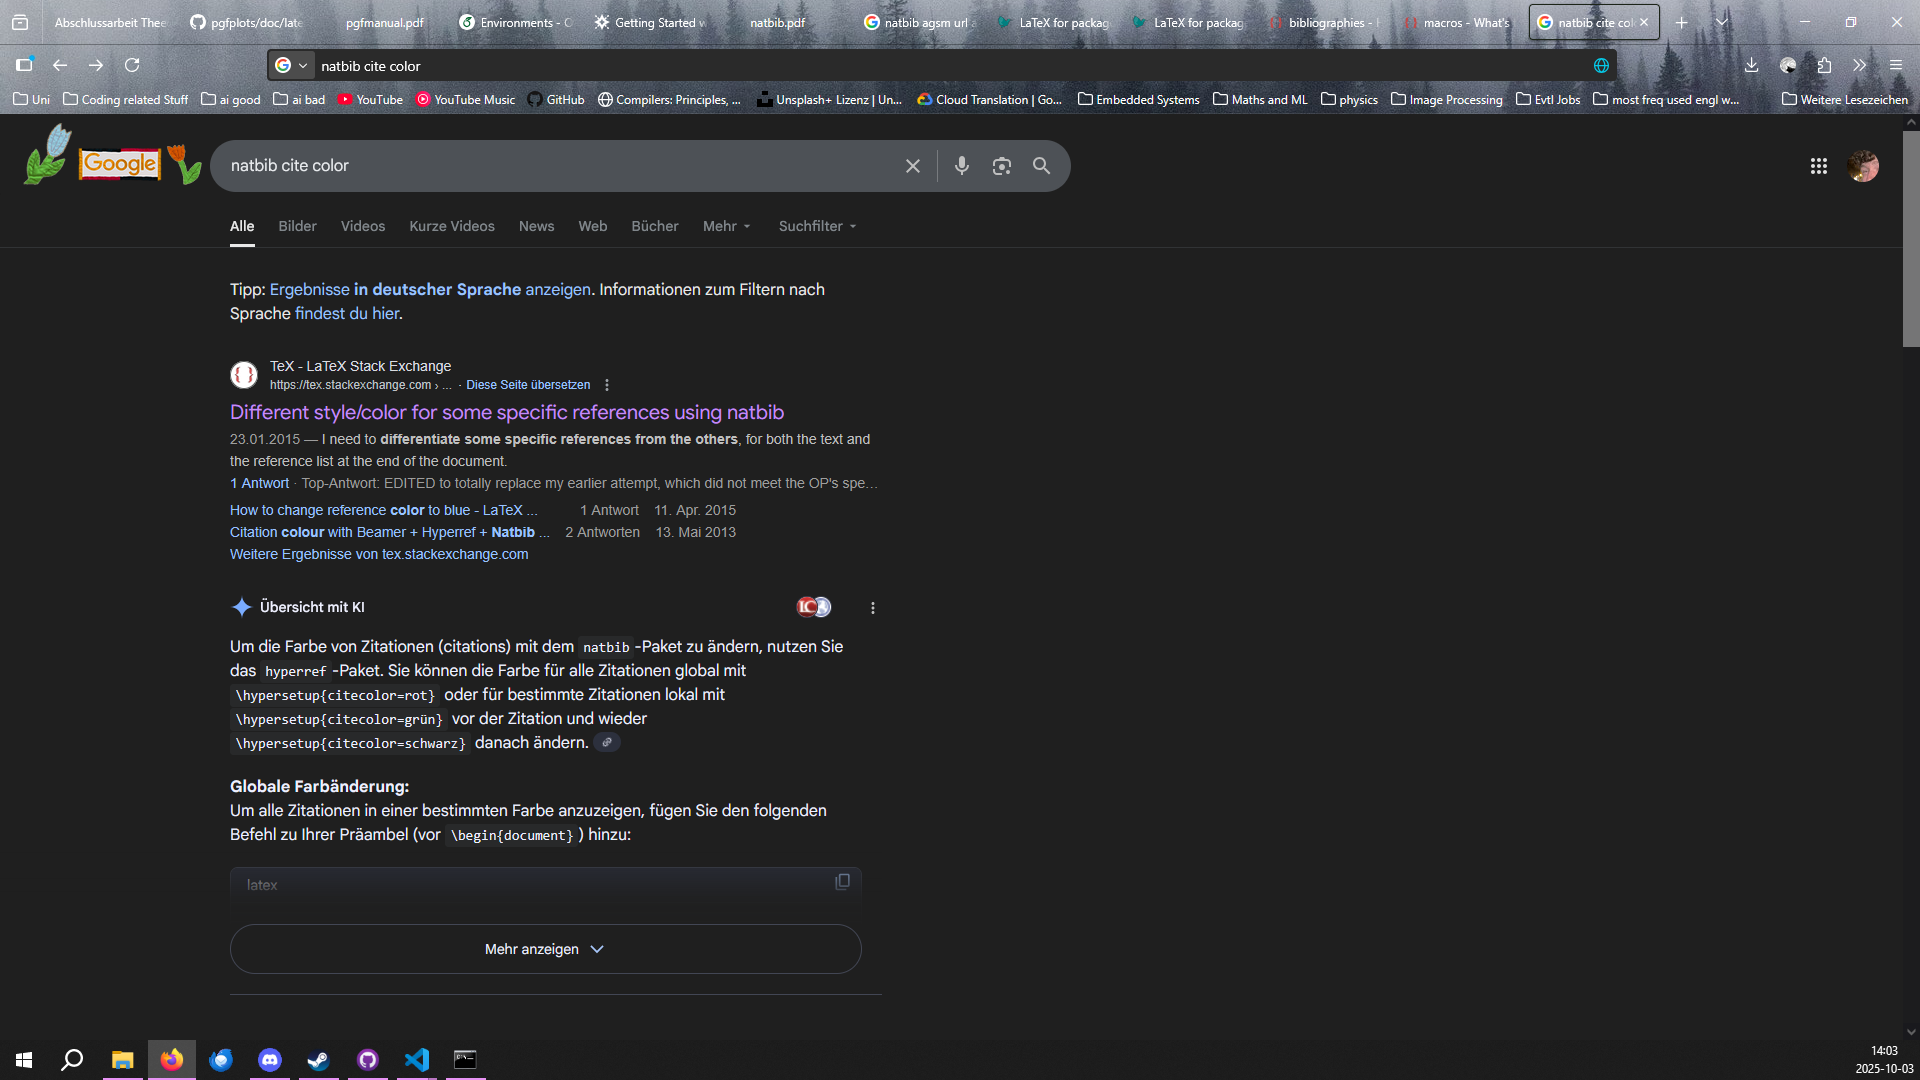
\includegraphics[width=\textwidth]{pictures/motivation.PNG}\label{fig:googlemakesmistakes}
\end{figure}